%%%%%%%%%%%%%%%%%%%%%%%%%%%%%%%%%%%%%%%%%%%%%%%%%%%%%%%%%%%%%%%%%%%%%%%%

%%% LaTeX Template for AAMAS-2027 (based on sample-sigconf.tex)
%%% Prepared from the official AAMAS-2027 submission instructions.

%%%%%%%%%%%%%%%%%%%%%%%%%%%%%%%%%%%%%%%%%%%%%%%%%%%%%%%%%%%%%%%%%%%%%%%%

%%% Start your document with the \documentclass command.


%%% == IMPORTANT ==
%%% Use the first variant below for the final paper (including author information).
%%% Use the second variant below to anonymize your submission (no author information shown).
%%% For further information on anonymity and double-blind reviewing, 
%%% please consult the call for paper information
%%% https://cyprusconferences.org/aamas2026/submission-instructions/

%%%% For anonymized submission, use this
\documentclass[sigconf,anonymous]{aamas}

%%%% For camera-ready, use this. Switching back also means restoring the
%%%% acknowledgements near the end of this file.
%\documentclass[sigconf]{aamas}


%%% Load required packages here (note that many are included already).

\usepackage{balance} % for balancing columns on the final page

%%%%%%%%%%%%%%%%%%%%%%%%%%%%%%%%%%%%%%%%%%%%%%%%%%%%%%%%%%%%%%%%%%%%%%%%

%%% AAMAS-2027 copyright block

\setcopyright{ifaamas}
\acmConference[AAMAS '27]{Proc.\@ of the 26th International Conference
on Autonomous Agents and Multiagent Systems (AAMAS 2027)}{May 3 -- 7, 2027}
{Hanoi, Vietnam}{AAMAS 2027 editors}
\copyrightyear{2027}
\acmYear{2027}
% \acmDOI{}
% \acmPrice{}
% \acmISBN{}


%%%%%%%%%%%%%%%%%%%%%%%%%%%%%%%%%%%%%%%%%%%%%%%%%%%%%%%%%%%%%%%%%%%%%%%%

%%%%%%%%%%%%%%%%%%%%%%%%%%%%%%%%%%%%%%%%%%%%%%%%%%%%%%%%%%%%%%%%%%%%%%%%

%%% Include any author-defined commands here.
         
\newcommand{\BibTeX}{\rm B\kern-.05em{\sc i\kern-.025em b}\kern-.08em\TeX}
\newcommand{\Safe}{\textsc{safe}}
\newcommand{\Unsafe}{\textsc{unsafe}}

%%%%%%%%%%%%%%%%%%%%%%%%%%%%%%%%%%%%%%%%%%%%%%%%%%%%%%%%%%%%%%%%%%%%%%%%

%%% == IMPORTANT ==
%%% Use this command to specify your submission number.
%%% In anonymous mode, it will be printed on the first page.

% Insert the assigned anonymous submission identifier after abstract registration.
% Leave empty in pre-registration builds so no placeholder appears in the PDF.
\newcommand{\SubmissionID}{}

\acmSubmissionID{\SubmissionID}

%%% Use this command to specify the title of your paper.

%\title[]{LLM Agents Underrepresent Human Strategic Diversity in AI Development Races}

\title[]{Supplementary Material: Humans Are More Diverse: Frontier LLMs Show Extreme Policies in Idealised AI Development Races}

%%% Provide names, affiliations, and email addresses for all authors.
% \author{Nimue}
% \affiliation{
%   \institution{The Lady's Lake}
%   \city{Avalon}
%   \country{United Kingdom}}
% \email{lady.of.the.lake@avalon.uk}

% \author{Phu-Hoa Pham}
% \affiliation{
%   \institution{Vietnam National University of Ho Chi Minh City}
%   \institution{Ho Chi Minh City University of Science}
%   \city{Ho Chi Minh City}
%   \country{Vietnam}}
% \email{23122030@student.hcmus.edu.vn}
% \author{Phu-Quy Nguyen-Lam}
% \affiliation{
%   \institution{Vietnam National University of Ho Chi Minh City}
%   \institution{Ho Chi Minh City University of Science}
%   \city{Ho Chi Minh City}
%   \country{Vietnam}}
% \email{23122048@student.hcmus.edu.vn}
% \author{Dao Sy Duy Minh}
% \affiliation{
%   \institution{Vietnam National University of Ho Chi Minh City}
%   \institution{Ho Chi Minh City University of Science}
%   \city{Ho Chi Minh City}
%   \country{Vietnam}}
% \email{23122041@student.hcmus.edu.vn}
% \author{Trung-Kiet Huynh}
% \affiliation{
%   \institution{Vietnam National University of Ho Chi Minh City}
%   \institution{Ho Chi Minh City University of Science}
%   \city{Ho Chi Minh City}
%   \country{Vietnam}}
% \email{23122039@student.hcmus.edu.vn}
% \author{Chi-Nguyen Tran}
% \affiliation{
%   \institution{Vietnam National University of Ho Chi Minh City}
%   \institution{Ho Chi Minh City University of Science}
%   \city{Ho Chi Minh City}
%   \country{Vietnam}}
% \email{23122044@student.hcmus.edu.vn}

% \author{Minh-Trung Le}
% \affiliation{
%   \institution{Ho Chi Minh City University of Technology (HCMUT)}
%   \institution{Vietnam National University Ho Chi Minh City (VNUHCM)}
%   \city{Ho Chi Minh City}
%   \country{Vietnam}}
% \email{trung.leminh@hcmut.edu.vn}
% \author{Phong-Hao Le}
% \affiliation{
%   \institution{Ho Chi Minh City University of Technology (HCMUT)}
%   \institution{Vietnam National University Ho Chi Minh City (VNUHCM)}
%   \city{Ho Chi Minh City}
%   \country{Vietnam}}
% \email{hao.lephong@hcmut.edu.vn}

% \author{Dinh-Nam Nguyen}
% \affiliation{
%   \institution{Ho Chi Minh City University of Technology (HCMUT)}
%   \institution{Vietnam National University Ho Chi Minh City (VNUHCM)}
%   \city{Ho Chi Minh City}
%   \country{Vietnam}}
% \email{nam.nguyenkhmt@hcmut.edu.vn}
% \author{Thien-Ky Nguyen-Dong}
% \affiliation{
%   \institution{Ho Chi Minh City University of Technology (HCMUT)}
%   \institution{Vietnam National University Ho Chi Minh City (VNUHCM)}
%   \city{Ho Chi Minh City}
%   \country{Vietnam}}
% \email{ky.nguyendongthien@hcmut.edu.vn}

% \author{Elias Fern\'andez Domingos}
% \affiliation{
%   \institution{Vrije Universiteit Brussel}
%   \institution{Universit\'e Libre de Bruxelles}
%   \city{Brussels}
%   \country{Belgium}}
% \email{elias.fernandez.domingos@vub.be}

% \author{Le Hong Trang}
% \affiliation{
%   \institution{Ho Chi Minh City University of Technology (HCMUT)}
%   \institution{Vietnam National University Ho Chi Minh City (VNUHCM)}
%   \city{Ho Chi Minh City}
%   \country{Vietnam}}
% \email{lhtrang@hcmut.edu.vn}

% \author{The Anh Han}
% \affiliation{
%   \institution{School of Computing, Engineering and Digital Technologies}
%   \institution{Center for Digital Innovation,  Teesside University}
%   \city{Middlesbrough}
%   \country{United Kingdom}}
% \email{T.Han@tees.ac.uk}


% =========================================================
% Reusable affiliations
% =========================================================

\newcommand{\HCMUSaffiliation}{%
  \affiliation{%
    \institution{Ho Chi Minh City University of Science}
    \institution{Vietnam National University Ho Chi Minh City (VNU-HCM)}
    \city{Ho Chi Minh City}
    \country{Vietnam}
  }%
}

\newcommand{\HCMUTaffiliation}{%
  \affiliation{%
    \institution{Ho Chi Minh City University of Technology (HCMUT)}
    \institution{Vietnam National University Ho Chi Minh City (VNU-HCM)}
    \city{Ho Chi Minh City}
    \country{Vietnam}
  }%
}

\newcommand{\BrusselsAffiliation}{%
  \affiliation{%
    \institution{Vrije Universiteit Brussel}
    \institution{Universit\'e Libre de Bruxelles}
    \city{Brussels}
    \country{Belgium}
  }%
}

\newcommand{\TeessideAffiliation}{%
  \affiliation{%
    \institution{School of Computing, Engineering and Digital Technologies}
    \institution{Center for Digital Innovation, Teesside University}
    \city{Middlesbrough}
    \country{United Kingdom}
  }%
}

% =========================================================
% Equal-contribution authors, listed alphabetically
% =========================================================
\author{Phu-Hoa Pham}
\authornotemark[1]
\HCMUSaffiliation
\email{23122030@student.hcmus.edu.vn}

\author{Duy-Minh Dao-Sy}
\authornote{These authors contributed equally to this work.}
\HCMUSaffiliation
\email{23122041@student.hcmus.edu.vn}

\author{Trung-Kiet Huynh}
\authornotemark[1]
\HCMUSaffiliation
\email{23122039@student.hcmus.edu.vn}

\author{Phu-Quy Nguyen-Lam}
\authornotemark[1]
\HCMUSaffiliation
\email{23122048@student.hcmus.edu.vn}



\author{Chi-Nguyen Tran}
\authornotemark[1]
\HCMUSaffiliation
\email{23122044@student.hcmus.edu.vn}
\author{Minh-Trung Le}
\authornotemark[1]
\HCMUTaffiliation
\email{trung.leminh@hcmut.edu.vn}

\author{Phong-Hao Le}
\authornotemark[1]
\HCMUTaffiliation
\email{hao.lephong@hcmut.edu.vn}

\author{Dinh-Nam Nguyen}
\authornotemark[1]
\HCMUTaffiliation
\email{nam.nguyenkhmt@hcmut.edu.vn}

\author{Thien-Ky Nguyen-Dong}
\authornotemark[1]
\HCMUTaffiliation
\email{ky.nguyendongthien@hcmut.edu.vn}



% =========================================================
% Corresponding authors, in the requested order
% =========================================================

\author{Elias Fern\'andez Domingos}
%\authornote{Corresponding authors.}
\BrusselsAffiliation
\email{elias.fernandez.domingos@vub.be}

\author{Le Hong Trang}
\authornote{Corresponding authors.}
%\authornotemark[2]
\HCMUTaffiliation
\email{lhtrang@hcmut.edu.vn}

\author{The Anh Han}
\authornotemark[2]
\TeessideAffiliation
\email{T.Han@tees.ac.uk}

%%% Use this environment to specify a short abstract for your paper.
\begin{abstract}
This document holds the material the main paper points to but has no room to
carry: the full breakdown of every task-validity probe, the replication check
against the human benchmark, a claim-by-claim audit of the citations, the
persona and measured-risk comparison, the predictive analysis behind the
reported drivers, and the complete descriptive baselines for two-player and
$N$-player races. Nothing here is needed to follow the main argument.
Everything here comes from the same runs, under the same admission rules, and
is reported at the same evidence level.
\end{abstract}

%%% Use this command to specify a few keywords describing your work.
%%% Keywords should be separated by commas.

% \keywords{Legends, Myths, Folktales}
\keywords{Large language models, AI development races, multi-agent systems, repeated games, AI safety, task validity}

%%%%%%%%%%%%%%%%%%%%%%%%%%%%%%%%%%%%%%%%%%%%%%%%%%%%%%%%%%%%%%%%%%%%%%%%

%%% Include any author-defined commands here.
         
% \newcommand{\BibTeX}{\rm B\kern-.05em{\sc i\kern-.025em b}\kern-.08em\TeX}

%%%%%%%%%%%%%%%%%%%%%%%%%%%%%%%%%%%%%%%%%%%%%%%%%%%%%%%%%%%%%%%%%%%%%%%%
\settopmatter{printacmref=false}
\renewcommand\footnotetextcopyrightpermission[1]{}
%\linespread{0.9}
\begin{document}
\maketitle

\section*{How to read this document}

Each section stands on its own and is named for what it measures. Section
letters restart at A because this is supplementary matter.

\begin{itemize}
  \item \textbf{Task-validity probe battery.} Every probe, its wording family,
    and the per-model pass rate behind the summary in the main paper.
  \item \textbf{Human-benchmark replication check.} Whether the reference
    human study's reported pattern reproduces on the released participant data
    under our own analysis code.
  \item \textbf{Claim-scoped citation audit.} For each cited work, the claim it
    is used to support and the claim it does not support.
  \item \textbf{Risk preference and assigned personas.} The persona families,
    and how a prompted persona compares with measured human risk preference.
  \item \textbf{Predictive structure of unsafe choices.} The feature analysis
    behind the drivers reported in the main paper.
  \item \textbf{Two-player descriptive baseline, full scope.} Every checkpoint
    and condition, including those the main paper does not plot.
  \item \textbf{$N$-player self-play scope.} Group sizes three to five.
  \item \textbf{Trajectory embedding recoloured by outcome.} The same
  embedding as the main paper, coloured by unsafe rate instead of population.
  \item \textbf{Unsafe rate by persona band and relative position.} The
    cell-level numbers behind the grouped-bar figure in the main paper.
\end{itemize}

\appendix
\section{Extended results and robustness checks}
\label{app:extended-results}
% NOTE: remove the \appendix command above if the surrounding paper already
% declares \appendix elsewhere (e.g. before the bibliography) -- it must
% appear exactly once in the document.

% Fallback definitions so this file compiles standalone or under a master
% file that has not defined these yet; \providecommand is a no-op if the
% surrounding document already defines them.
\providecommand{\Safe}{\textsc{Safe}}
\providecommand{\Unsafe}{\textsc{Unsafe}}
\providecommand{\todo}[1]{\textbf{[TODO: #1]}}

This appendix collects the material referenced from
the results section in the main paper as supporting rather than extending the main
claims: the full task-validity probe breakdown
(\S\ref{app:task-validity-full}), the human-benchmark replication check
(\S\ref{app:human-benchmark-replication}), the persona comparison
(\S\ref{app:persona-detail}), the predictive analysis
(\S\ref{app:predictive-structure}), and the full two-player and $N$-player
descriptive results (\S\ref{app:twoplayer-baseline},
\S\ref{app:nplayer-scope}).

\subsection{Task-validity probe battery: full breakdown}
\label{app:task-validity-full}

Table~\ref{tab:task-validity-full} reports the full breakdown behind the
frontier endpoint admission in the main paper. The confirmatory audit used the
the two exact routes listed in Table~\ref{tab:frontier-admission-registry} under
the frozen protocol v5: 20 atomic probes spanning rule recall,
one-stage payoffs, state reconstruction, state transition, terminal scoring,
and expected payoff, repeated three times per route for 120 retained outputs.
Every response was schema-valid and no transport retry was needed. Numeric
probes used a fixed structured-output contract; categorical probes explicitly
listed the allowed answer set.

\begin{table}[h]
    \caption{Task-validity probe accuracy by category for the two admitted
    frontier routes, protocol v5 ($n=60$
    retained probe outputs per route).}
    \label{tab:task-validity-full}
    \centering
    \small
        \begin{tabular}{@{}lrr@{}}
        \toprule
        Probe category & Gemini 3 Flash & Claude Sonnet 5 \\
        \midrule
        Rule recall                        & 100.0\% & 100.0\% \\
        One-stage payoff lookup             & 100.0\% & 100.0\% \\
        State reconstruction                & 93.3\% & 86.7\% \\
        State transition                    & 100.0\% & 100.0\% \\
        Terminal scoring                    & 100.0\% & 80.0\% \\
        Expected-payoff calculation         & 50.0\% & 0.0\% \\
        \midrule
        \emph{Overall semantic accuracy}    & \emph{93.3\%} & \emph{81.7\%} \\
        \emph{Schema-valid responses}      & \emph{100.0\%} & \emph{100.0\%} \\
        \bottomrule
    \end{tabular}
\end{table}

The largest errors were in the optional payoff check: three of six Gemini
responses and none of the Claude responses were correct. We retain this domain
as a diagnostic. Live gameplay asks for an action, whereas the state and
terminal domains determine whether the action prompt is mechanically interpretable.
The admission task therefore records both the required gate and the arithmetic
limitation instead of silently dropping the endpoint.

\subsection{Frontier endpoint registry and admission outcomes}
\label{app:frontier-admission}

Endpoint availability was checked against the active Kaggle Benchmark identity
and recorded using the exact route string. One repetition of the 20-probe
bank was used as a diagnostic smoke for every advertised route; the two routes
that passed the v5 gameplay thresholds then received the three-repetition
confirmatory admission. A route that was unavailable or failed transport was
retained as failed infrastructure evidence, never replaced by another
endpoint.

\begin{table}[h]
    \caption{Per-endpoint frontier admission audit. Smoke results are
    diagnostic; only routes with a completed v5 artifact and passing gameplay
    thresholds enter the new gameplay run.}
    \label{tab:frontier-admission-registry}
    \centering
    \scriptsize
    \begin{tabular}{@{}p{0.44\linewidth}rrrp{0.12\linewidth}@{}}
        \toprule
        Exact route & Overall & State & Terminal & Status \\
        \midrule
        \path{google/gemini-3-flash-preview} & 93.3\% & 93.3\% & 100\% & admitted \\
        \path{anthropic/claude-sonnet-5@default} & 81.7\% & 86.7\% & 80\% & admitted \\
        \path{google/gemini-3.1-flash-lite-preview} & 75\% & 60\% & 80\% & diagnostic \\
        \path{openai/gpt-5.4-nano-2026-03-17} & 50\% & 20\% & 60\% & diagnostic \\
        \path{deepseek-ai/deepseek-r1-0528} & \multicolumn{3}{c}{not admitted} & transport failed \\
        \path{ibm/granite-4.0-h-small} & \multicolumn{3}{c}{not admitted} & transport failed \\
        \path{openai/gpt-oss-120b} & \multicolumn{3}{c}{not admitted} & transport failed \\
        \path{qwen/qwen3-next-80b-a3b-instruct} & \multicolumn{3}{c}{not admitted} & transport failed \\
        \bottomrule
    \end{tabular}
\end{table}

The required gameplay gate was overall accuracy at least 80\%, state
reconstruction accuracy at least 75\%, and terminal-scoring accuracy at least
75\%. Expected-payoff accuracy was reported separately because it is a
closed-form arithmetic diagnostic rather than an action-task requirement.
The active identity exposed no second authorised account, so no multi-account
pooling is claimed.

\subsection{Frontier neutral baseline}
\label{app:frontier-baseline}

The new neutral gameplay baseline used protocol v3, the same mechanism and
prompt for both admitted routes, ten repetitions per risk level, and 30 races
per route. Each
route produced 558 structured decisions with zero parse failures. The entries
in Table~\ref{tab:frontier-baseline} are decision-weighted Unsafe rates; they
are not pooled across routes and do not estimate an evolutionary equilibrium.

\begin{table}[h]
    \caption{Neutral two-player frontier baseline under the admitted routes.
    Each route has 30 races, 558 decisions, and zero parse failures.}
    \label{tab:frontier-baseline}
    \centering
    \scriptsize
    \begin{tabular}{@{}p{0.43\linewidth}rrrp{0.12\linewidth}@{}}
        \toprule
        Exact route & $r=.1$ & $r=.6$ & $r=.9$ & Races \\
        \midrule
        \path{google/gemini-3-flash-preview} & 98.9\% & 74.2\% & 59.1\% & 30 \\
        \path{anthropic/claude-sonnet-5@default} & 89.2\% & 46.2\% & 37.6\% & 30 \\
        \bottomrule
    \end{tabular}
\end{table}

The Gemini manifest records that the hosted SDK stripped the requested
sampling seed. The Claude manifest records that the seed was forwarded but
provider-side application was not confirmed. Temperature was requested as
0.7 for both routes but was not forwarded by this SDK path. These facts bound
the result to the exact hosted route and software contract.

To make the comparison boundary explicit, Figure~\ref{fig:egt-frontier-insights}
separates the risk response, the route-specific departure from the strong-
selection reconstruction, the nearest-rule diagnostic, and its mismatch
rate. This is an analysis artifact rather than an equilibrium test: the
frontier routes generate prompted self-play trajectories, whereas EGT samples
stationary population composition.

\begin{figure*}[t]
    \centering
    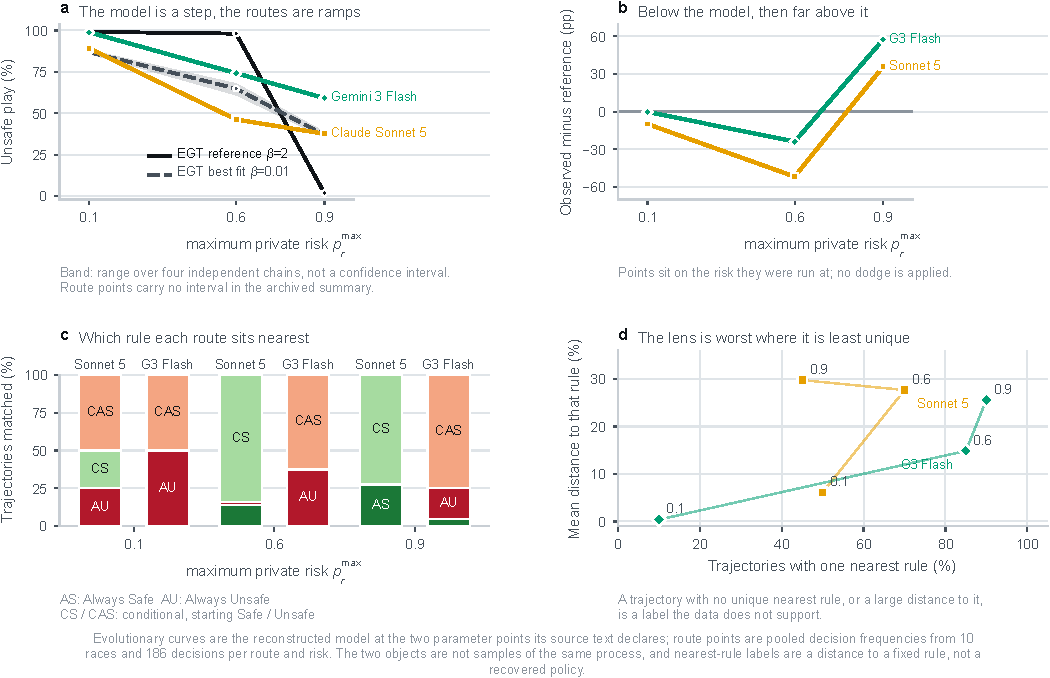
\includegraphics[width=\textwidth]{../figures/paper/egt_frontier_insights.pdf}
    \caption{Boundary analysis for the reconstructed evolutionary model and
    the two admitted frontier routes. Panel A shows route-specific Unsafe
    responses alongside the two EGT parameter regimes. Panel B shows the
    deviation from the strong-selection EGT reference. Panel C gives the
    nearest-rule composition, and Panel D shows why those labels are only a
    diagnostic lens: uniqueness and minimum mismatch vary across routes and
    risk levels.}
    \Description{Four-panel figure comparing evolutionary-game theory with
    Gemini and Claude frontier self-play. The panels show risk responses,
    deviations from theory, nearest-rule compositions, and classification
    mismatch against uniqueness.}
\label{fig:egt-frontier-insights}
\end{figure*}

The invasion view in Figure~\ref{fig:egt-frontier-invasion} exposes the
selection topology behind the three theoretical endpoints. Its directed edges
are computed by the archive-compatible EGTtools implementation. The node areas
use the finite-mutation main-reference chain because the small-mutation limit
can contain multiple absorbing classes at extreme payoff scales. This is a
diagnostic decomposition, not a claim that the frontier routes sample the same
population process.

\begin{figure*}[t]
    \centering
    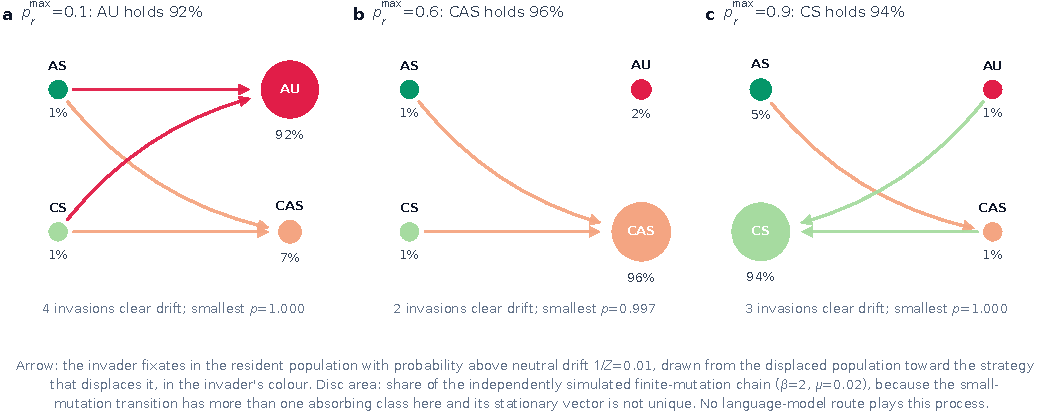
\includegraphics[width=\textwidth]{../figures/paper/egt_frontier_invasion.pdf}
    \caption{Risk-conditioned invasion topology for the reduced evolutionary
    game. Node area shows the finite-mutation main-reference chain share
    ($\beta=2$, $\mu=0.02$); directed edges show EGTtools
    \texttt{PairwiseComparison} fixation probabilities above neutral drift.
    The figure is a hybrid diagnostic: the edge topology is evaluated in the
    EGTtools small-mutation limit, while node areas come from the independently
    simulated finite-mutation chains. It should not be read as a latent-strategy
    diagram for the language models.}
    \Description{Three network diagrams showing risk-conditioned invasion among
    Always Safe, Always Unsafe, Conditional Safe, and Conditional Unsafe.
    Node areas show finite-mutation stationary shares, and arrows show
    EGTtools fixation probabilities above neutral drift.}
    \label{fig:egt-frontier-invasion}
\end{figure*}

\subsection{Human-benchmark replication check}
\label{app:human-benchmark-replication}

Before comparing model-generated behaviour with the human benchmark of
\citet{falling_behind_unsafe} in the two-player strategic diversity results in the main paper, we first
validated our reconstruction of that benchmark by refitting its published
dynamic specification on the same public de-identified data. The
reconstructed estimation sample contains 2{,}888 round-level observations,
172 race-pair clusters, and 338 participants. Table~\ref{tab:human-replication} compares the refit coefficients against the values reported in the
original study.

\begin{table}[h]
    \caption{Replication of \citet{falling_behind_unsafe}'s dynamic
    specification on the public de-identified human data. ``Reconstructed''
    is our refit; ``Original'' is the coefficient reported in the source
    study.}
    \label{tab:human-replication}
    \centering
    \small
    \begin{tabular}{@{}lrr@{}}
        \toprule
        Term & Reconstructed & Original \\
        \midrule
        Opponent's previous action & 0.606  & 0.607  \\
        Player's progress gap      & $-0.295$ & $-0.296$ \\
        First-round action         & 0.217  & 0.217  \\
        Player's own previous action & $-0.195$ & $-0.193$ \\
        \bottomrule
    \end{tabular}
\end{table}

\subsection{Claim-scoped citation audit}
\label{app:citation-audit}

Table~\ref{tab:citation-audit} records both the supported use of each cited
study and the nearest excluded overclaim. These evidence boundaries do not
turn the diagnostic pilots in this paper into confirmatory results.

\begin{table*}[t]
\caption{Source-level audit for citations added to the prompt-sensitivity
and behavioural-validity argument.}
\label{tab:citation-audit}
\small
\begin{tabular}{@{}p{0.16\textwidth}p{0.38\textwidth}p{0.38\textwidth}@{}}
\toprule
Source & Supported use & Excluded overclaim \\
\midrule
Sclar et al.~\citep{sclarPromptFormatting2024} &
Meaning-preserving few-shot formatting changes can yield large,
model-dependent performance spreads. &
Not evidence for semantic paraphrase effects or a universal effect size. \\
Pezeshkpour and Hruschka~\citep{pezeshkpourOptionOrder2024} &
Reordering multiple-choice answer options can change predictions. &
The proposed uncertainty-plus-placement mechanism is not causally
identified. \\
Wei et al.~\citep{weiSelectionBias2024} &
Order and response-token identity are distinct selection-bias targets. &
Not proof that every task or model exhibits the same bias. \\
Salinas and Morstatter~\citep{salinasButterfly2024} &
Controlled output-format and atomic whitespace variants can alter answers. &
Not a claim that every added space changes behaviour. \\
Zheng et al.~\citep{zhengPersona2024} &
Across their factual-question setup, average persona benefit was absent or
slightly negative and reliable persona selection remained difficult. &
Not a universal null effect for persona-driven agent tasks. \\
Aher et al.~\citep{using_llm_to_simulate} &
Three of four behavioural findings were qualitatively reproduced, while the
fourth showed a hyper-accuracy distortion. &
Not evidence that LLM samples are interchangeable with human populations. \\
Akata et al.~\citep{playing_repeated_games_with_llms} &
Prediction before action improved coordination and scores in repeated games. &
Not a general claim that an observed action reveals a correct opponent
belief. \\
Herr et al.~\citep{herrStrategicBias2024} &
Action-label order and payoff reassignment changed choices in two canonical
two-player games. &
Not evidence that every strategically equivalent transformation has the same
effect. \\
Robinson and Burden~\citep{robinsonBurdenFraming2025} &
Procedurally varied vignettes produced substantial contextual variability
under one underlying Prisoner's Dilemma structure. &
Not a repeated-game result and not an estimate for the present race. \\
Wu et al.~\citep{wuCounterfactual2024} &
Performance declined consistently across 11 tasks when default mappings were
replaced by specified counterfactual alternatives. &
Not proof that the tested models lacked all abstract reasoning ability. \\
del Rio-Chanona et al.~\citep{delRioChanonaMarkets2025} &
LLM markets recovered broad feedback-condition dynamics but displayed less
strategy heterogeneity than human participants. &
Not evidence that LLM agents and human participants are exchangeable. \\
\bottomrule
\end{tabular}
\end{table*}

The reconstruction reproduces the original coefficients almost exactly
(largest discrepancy 0.002), which is the basis for treating the human-side
comparisons in the two-player strategic diversity results in the main paper and
the persona and measured risk results in the main paper as resting on a correctly processed benchmark
rather than on a reimplementation error.

\subsection{Risk preference and assigned personas}
\label{app:persona-detail}


We finally distinguish three constructs that should not be conflated: the
human participants' pre-game elicited risk preference, the mechanism's
assigned private-risk treatment, and the narrative risk persona supplied to
an LLM in its prompt. Human participants completed an incentivised
Eckel--Grossman gamble elicitation (0 = most risk-averse, 5 = least
risk-averse) before playing the two-player race. This elicited measure has
essentially no direct association with subsequent \Unsafe{} rate,
\[
    \text{slope}=-0.004,\qquad r=-0.015,\qquad p=0.79,\qquad n=341,
\]
with the difference in mean \Unsafe{} play between the most and least
risk-accepting human groups (approximately five percentage points) lying
within the corresponding uncertainty interval. This null result
independently reproduces \citeauthor{falling_behind_unsafe}'s own
preregistered finding that elicited risk preference did not significantly
predict \Unsafe{} choice \citep{falling_behind_unsafe}, and stands in
contrast to the tournament literature's general finding that human
risk-taking responds to competitive standing rather than remaining a fixed
trait \citep{risk-taking_touraments,risk_taking_in_competition,%
competition_and_risk-taking}: in this task, the round-by-round interaction
captured in the two-player strategic diversity results in the main paper
is a stronger organising signal than static pre-game disposition. The
multiplayer position analysis is exploratory and is not used as a second
independent confirmation of this two-player result. A
weaker, second-order association does survive at the level of behavioural
phenotype rather than mean rate: the same elicited measure differs across
the raw-sequence archetypes of the two-player strategic diversity results in the main paper (Kruskal--
Wallis $H=21.95$, $p=0.001$, $n=286$ clustered human players), so the
elicitation may help stratify \emph{which} dynamic pattern a participant
falls into even though it does not predict \emph{how much} \Unsafe{} they
play overall.

\begin{figure*}[t]
    \centering
    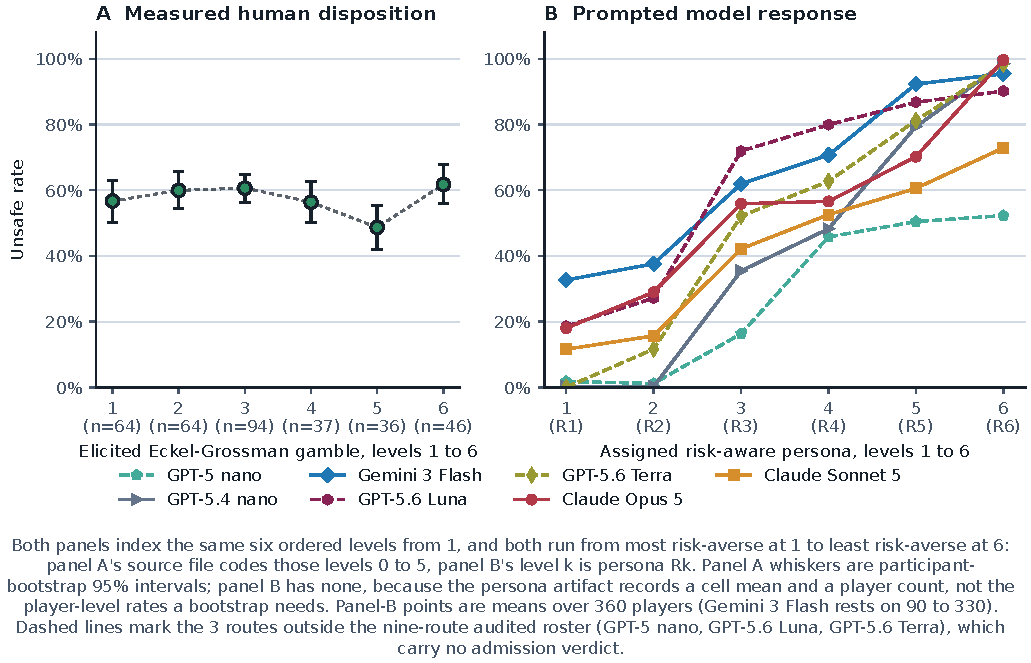
\includegraphics[width=\textwidth]{../figures/paper/llm_human_clustering/09_human_vs_llm_own_risk_dependence.pdf}
    \caption{A measured human disposition against an assigned model label.
    Left: mean \Unsafe{} rate by elicited Eckel--Grossman gamble choice,
    with 95\% confidence intervals and participants per bin; the dotted
    line is the trend across the six group means. Right: mean \Unsafe{}
    rate by assigned risk-persona level, for every model with a six-level
    sweep; GPT-5.6 Luna and Terra (dashed) are the two routes outside the
    main baseline roster. The shared six-step axis is visual alignment only;
    the left is a disposition measured once before play, the right an
    instruction re-assigned every race.}
    \label{fig:own-risk-dependence}
    \Description{Two panels sharing a vertical Unsafe-rate axis and a
    six-step horizontal axis. The left panel plots human mean Unsafe rate
    against the elicited Eckel-Grossman gamble choice from 0 to 5, with 95
    percent confidence intervals and the number of participants beneath
    each point; the six points stay between 0.49 and 0.62 and a dotted
    trend line through them is almost flat. The right panel plots mean
    Unsafe rate against the assigned risk-persona level R1 to R6 for seven
    models, each with its own colour and marker shape. Every model line
    climbs steeply from left to right, from near the floor or lower middle
    at R1 to between 0.52 and 1.0 at R6; the two GPT-5.6 lines are dashed
    because they are outside the main baseline roster.}
\end{figure*}

Figure~\ref{fig:own-risk-dependence} (left) shows how little that null
leaves. Human mean \Unsafe{} play stays inside a 49--62\% band across the
entire elicitation range, never approaching the low-\Unsafe{} models of
the two-player strategic diversity results in the main paper (GPT-5-nano 17\%, Claude Sonnet 5 22\%,
Claude Opus 5 33\%) or the high-\Unsafe{} Gemini models (73--83\%).
Elicited risk preference does not move a participant far enough to resemble
a different model's policy.

The right panel is the opposite (Table~\ref{tab:persona-effect}): every
model with a six-level sweep climbs 50.5 to 98.3 points from R1 to R6, all
but the two nano models monotonically, and those two dip by well under a
point at R2 before rising. The label does not, however, move models by a
common factor; GPT-5.6 Terra runs lowest at R1 and finishes within 1.3
points of the top, while GPT-5-nano starts fifth of seven and ends last
last, so curve order is not preserved, and the same instruction is worth
very different amounts to different models. Of the seven tested models, five have such a sweep;
neither Gemini Flash-Lite checkpoint does. In logistic models that
additionally control for the mechanism's actual private-risk treatment, the
coefficients on the agent's own assigned risk label remain large for the
three models where that controlled fit has been run, so the persona effect
is not simply standing in for the mechanical risk treatment.

\begin{table}[t]
    \caption{LLM risk-persona effect: change in \Unsafe{} rate from the
    lowest (R1) to the highest (R6) assigned risk label, and the per-level
    OLS slope, for every model with a six-level risk-label sweep ($n=360$
    players per level, $n=330$ for Gemini-3-Flash). The persona coefficient
    (logistic model additionally controlling for the mechanism's actual
    private-risk treatment) has been fit only for the first three; ``not
    estimated'' marks models for which only the descriptive delta and slope are
    available. Starred rows sit outside the seven-model roster.}
    \label{tab:persona-effect}
    \centering
    \small
    \begin{tabular}{@{}lrrr@{}}
        \toprule
        Model & $\Delta$ \Unsafe{} (pp) & Per-level slope & Coefficient \\
        \midrule
        GPT-5-nano       & 50.5 & 0.123 & 0.93 \\
        GPT-5.4-nano     & 98.2 & 0.212 & 1.47 \\
        Gemini-3-Flash   & 62.8 & 0.139 & 2.03 \\
        Claude Opus 5    & 81.6 & 0.152 & not estimated \\
        Claude Sonnet 5  & 61.3 & 0.129 & not estimated \\
        GPT-5.6 Luna$^*$  & 71.5 & 0.156 & not estimated \\
        GPT-5.6 Terra$^*$ & 98.3 & 0.203 & not estimated \\
        \bottomrule
    \end{tabular}
\end{table}

This contrast does not show that LLM agents possess a latent risk
preference comparable to the human elicitation: the human variable is a
measured pre-game disposition that turns out to be nearly unrelated to
in-game behaviour, whereas the LLM variable is an explicit instruction
embedded in the prompt. The more defensible reading is that an assigned
risk persona functions as a high-salience behavioural instruction for
these models, not as an analogue of a stable human risk
disposition. Because the LLM estimates come from a separate risk-matrix
experiment, available for five of the seven tested models and with the
private-risk-controlled logistic fit run for only three of those five,
this comparison remains exploratory and cross-experimental rather than a
like-for-like measurement.

\subsection{Population identity in first-five-round trajectories}
\label{app:population-identity}

The population-identity diagnostic in the main paper uses the same 15 raw
features as the trajectory visualisation. We fit a shallow decision tree with
class-balanced loss under stratified five-fold grouped cross-validation. The
two seats of an LLM race remain in the same fold; human observations are
grouped by participant. Since the pooled classes are unequal, balanced
accuracy and macro-F1 are the primary measures. A 200-repetition permutation
null preserves the observed class counts and the same folds.

\begin{table}[t]
    \caption{Race-grouped population-identity diagnostic on 760 complete
    first-five-round trajectories. The eight populations are imbalanced
    (340 human and 60 per checkpoint), so balanced accuracy and macro-F1 are
    primary. The null interval is the 2.5--97.5 percentile range over grouped
    label permutations.}
    \label{tab:population-identity}
    \centering
    \scriptsize
    \setlength{\tabcolsep}{3pt}
    \resizebox{\columnwidth}{!}{%
    \begin{tabular}{@{}lccc@{}}
        \toprule
        Metric & Observed & Permutation null mean & Null 95\% interval \\
        \midrule
        Raw accuracy & 0.292 $\pm$ 0.053 & 0.086 & 0.039--0.178 \\
        Balanced accuracy & \textbf{0.423 $\pm$ 0.043} & 0.124 & 0.070--0.182 \\
        Macro-F1 & \textbf{0.252 $\pm$ 0.047} & 0.063 & 0.025--0.112 \\
        \bottomrule
    \end{tabular}
    }
\end{table}

The balanced accuracy exceeds the class-balanced chance level of $1/8$ and
the grouped permutation null ($p<0.001$); raw accuracy is shown only for
completeness because it is affected by the large human class. This result
supports observable differences in the first-five-round trajectories, while
the overlap and the shallow classifier do not support a claim that a latent
strategy or model identity is cleanly recoverable. The machine-readable
result and source hashes are stored in
\texttt{results/cross\_model\_pilot\_synthesis/data/}.

\subsection{Predictive structure of \Unsafe{} choices}
\label{app:predictive-structure}

The preceding section shows that populations produce different action
patterns. We now ask which recorded parts of the game best predict their next
Unsafe choice. This is a study of association, not cause or internal
reasoning. For each population, we fit a random forest, a model that combines
many decision trees. Predictive scores use five-fold grouped cross-validation,
with all decisions from one participant or race kept in one fold. The forest
predicts decisions after round one from five values
known before the choice: the player's previous action, the opponent's previous
action, the progress gap, the assigned maximum private risk, and the round
number. TreeSHAP then measures how much each value contributes to the fitted
model's predictions. A larger SHAP share means that the predictor relied more
on that feature. It does not mean that the feature caused the decision.

\begin{figure}[t]
    \centering
    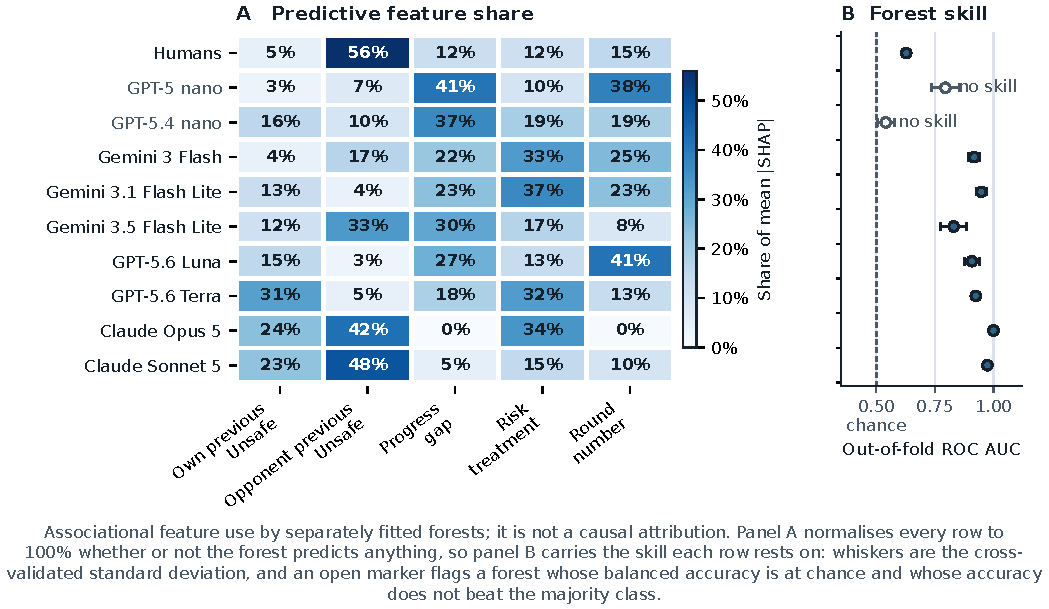
\includegraphics[width=0.95\linewidth]{../figures/paper/llm_human_clustering/feature_importance_shap_heatmap.pdf}
    \caption{Population-specific predictive structure for round-$t\geq2$
    \Unsafe{} choices. Each row reports the share of mean absolute SHAP
    value assigned to the same five pre-decision features by a random
    forest fitted separately to that population. SHAP magnitudes describe
    how the fitted classifier uses observed features; they are neither
    causal effects nor evidence of the agents' internal reasoning.}
    \label{fig:feature-importance}
    \Description{Heatmap of the share of mean absolute SHAP value that a
    random forest assigns to each of five pre-decision features, with one
    row per population and one column per feature: own previous action,
    opponent's previous action, progress gap, assigned risk treatment, and
    round number. The human row is dominated by the opponent's previous
    action at 56 percent. GPT-5-nano is dominated instead by progress gap
    and round number at 41 and 38 percent, the two Gemini Flash checkpoints by
    the risk treatment at 33 and 37 percent, and Claude Sonnet 5 by the
    opponent's previous action at 48 percent.}
\end{figure}

\begin{table*}[t]
    \caption{Population-specific random-forest prediction of \Unsafe{}
    play. Feature columns report shares of total mean absolute SHAP
    magnitude (rows sum to 100\%, up to rounding); AUC and balanced
    accuracy are mean out-of-fold values from the population-specific
    race/participant-grouped five-fold split.}
    \label{tab:feature-importance}
    \centering
    \footnotesize
    \setlength{\tabcolsep}{4.5pt}
    \begin{tabular}{@{}lrrrrrrr@{}}
        \toprule
        Population
        & Own previous
        & Opponent previous
        & Progress gap
        & Risk
        & Round
        & OOF AUC
        & Balanced accuracy \\
        \midrule
        Human                   & 5\%  & \textbf{56\%} & 12\% & 12\%          & 15\% & 0.63 & 0.58 \\
        GPT-5-nano              & 3\%  & 7\%           & \textbf{41\%} & 10\% & 38\% & 0.80 & 0.50 \\
        GPT-5.4-nano            & 16\% & 10\%          & \textbf{37\%} & 19\% & 19\% & 0.54 & 0.52 \\
        Gemini-3-Flash          & 4\%  & 17\%          & 22\% & \textbf{33\%} & 25\% & 0.92 & 0.77 \\
        Gemini-3.1-Flash-Lite   & 13\% & 4\%           & 23\% & \textbf{37\%} & 23\% & 0.95 & 0.75 \\
        Gemini-3.5-Flash-Lite   & 12\% & \textbf{33\%} & 30\% & 17\%          & 8\%  & 0.83 & 0.71 \\
        Claude Opus 5           & 24\% & 42\%$^\dagger$ & 0\% & 34\%         & 0\%  & 1.00 & 1.00 \\
        Claude Sonnet 5         & 23\% & \textbf{48\%} & 5\%  & 15\%          & 10\% & 0.97 & 0.93 \\
        \bottomrule
    \end{tabular}

    \vspace{2pt}
    {\footnotesize $^\dagger$Collinear with the risk treatment, not a
    reciprocity estimate; see the discussion below.\par}
\end{table*}

For human participants, the opponent's previous action accounts for 56\%
of total SHAP magnitude, far more than any other feature, while the
player's own previous action contributes only 5\%: a reciprocity-dominated
profile that independently recovers the pattern found in the human
logistic analysis. GPT-5-nano is close to the opposite profile: relative
race position (progress gap) accounts for 41\% of its predictive
importance and opponent history for only 7\%, and its apparently strong
out-of-fold AUC of 0.80 is misleading on its own, since balanced accuracy is
exactly 0.50: the model plays so close to the \Safe{} floor that the
classifier effectively fails to recover the rare \Unsafe{} class. Gemini-3-
Flash and Gemini-3.1-Flash-Lite are primarily risk-treatment-driven (33\%
and 37\% of SHAP magnitude), consistent with their strong, monotone
descriptive risk-response curves. Claude Sonnet 5 is the only model whose
profile matches the human ordering outright, with the opponent's previous
action largest at 48\%, below the human 56\%;
Gemini-3.5-Flash-Lite is the next closest (33\%), though its progress gap
remains more influential than in the human model. GPT-5.4-nano has no
comparably dominant predictor: importance is
spread across progress gap, risk, round, and its own previous action,
with opponent history at 10\% and the lowest above-chance predictive
fit in the table (AUC 0.54, balanced accuracy 0.52), so its behaviour is
comparatively difficult to reconstruct from these five mechanical state
variables rather than clearly governed by any one signal.

Claude Opus 5 shows why these shares must be read against the design that
produced them. Its 42\% opponent share reads as strong reciprocity and is
not: on the neutral lane it plays \Unsafe{} on essentially every low-risk
decision and essentially none at high risk, so the risk treatment alone
separates its choices, and since both seats behave that way the opponent's
previous action is a proxy for the risk level rather than an independent
signal. The forest then splits importance between two variables encoding
the same event, and the perfect AUC describes a step function, not a better
fit. A feature-importance share is interpretable only where the feature
keeps variation independent of the others, which is what a
near-deterministic policy removes.

Predictive performance varies substantially across populations (AUC 0.54
to 1.00), so SHAP shares should not be read as directly comparable measures
of decision quality; floor and ceiling behaviour mechanically limits
minority-class prediction for several models. The defensible
conclusion is narrower than ``LLMs use different features'': the same
observable state variables organise predictive information differently
across populations, and matching a human aggregate action rate does not
imply matching the human reciprocity-dominated association profile.


% \subsection{HDBSCAN hyperparameter sensitivity and archetype composition}
% \label{app:hdbscan-sweep}

% The raw-action clustering summarised in the two-player strategic diversity results in the main paper
% (minimum cluster size 15, minimum samples 6, Euclidean distance,
% excess-of-mass selection) identifies eleven dense archetypes and leaves 98
% of 760 trajectories unclustered (12.9\%). The two largest archetypes anchor
% opposite ends of the space: a mutual-first-round-\Safe{} archetype
% ($n=138$) and a mutual-round-2-\Unsafe{} archetype ($n=124$); the remaining
% nine archetypes capture smaller switching and response patterns between
% these two poles.

% Because the number of clusters HDBSCAN recovers is data-dependent rather
% than fixed in advance, a hyperparameter sensitivity sweep (varying minimum
% cluster size and minimum samples around the values above) is the
% appropriate check on how much the eleven-archetype description depends on
% that specific configuration. \todo{No such sweep has been run and retained
% under this project's run-provenance policy: the clustering script
% currently hard-codes a single configuration
% (\texttt{min\_cluster\_size=15}, \texttt{min\_samples=6}) with no
% parameter loop or sweep manifest. An earlier draft of this paragraph
% reported a five-configuration sweep result (4--14 clusters, 35.5\%--61.4\%
% unclustered) that does not correspond to any artifact in the retained
% analysis outputs and has been removed rather than repeated here. Before
% this subsection can report a sensitivity range, implement and run a small
% grid (e.g.\ minimum cluster size and minimum samples each varied around
% 15/6) with its own manifest, and report the recovered cluster count and
% unclustered fraction per configuration from that manifest.}

\subsection{Two-player checkpoint descriptive baseline (full scope)}
\label{app:twoplayer-baseline}

The five-checkpoint two-player descriptive baseline referenced throughout
the two-player strategic diversity results in the main paper and the observable drivers of unsafe play in the main paper completed 150
races and 2{,}790 decisions, crossing five checkpoints (GPT-5-nano,
GPT-5.4-nano, Gemini-3-Flash-preview, Gemini-3.1-Flash-Lite,
Gemini-3.5-Flash-Lite) with the mechanism's three assigned private-risk
levels ($0.10,0.60,0.90$; Eq.~(2)). At the level of
descriptive curves rather than the pooled aggregate rates already reported
in the main text, GPT-5-nano's \Unsafe{} rate was low and nearly flat
across the three risk levels; GPT-5.4-nano's response to risk level was
non-monotone; and the three Gemini checkpoints' \Unsafe{} rate declined as
the assigned maximum risk increased -- the opposite direction from the two
OpenAI checkpoints. Because provider routes, protocol signatures, and pilot
sample sizes differ across checkpoints, these five curves demonstrate
qualitative heterogeneity in how each checkpoint responds to the risk
manipulation; we do not pool them into a single model-family estimate, and
the formal test of that heterogeneity is the checkpoint-by-risk interaction
reported in the two-player strategic diversity results in the main paper
($\chi^2(10)=354.7$, with a convergence warning, so only the conservative
$p<10^{-3}$ threshold is used in the main text).
Table~\ref{tab:twoplayer-baseline-full} gives the per-checkpoint,
per-risk-level rates underlying the qualitative curve descriptions above.

\begin{table}[h]
    \caption{Player-level \Unsafe{} rate by checkpoint and assigned
    maximum-private-risk level, five-checkpoint two-player descriptive
    baseline ($n=20$ players per checkpoint--risk cell, ten races each).}
    \label{tab:twoplayer-baseline-full}
    \centering
    \small
    \begin{tabular}{@{}lrrr@{}}
        \toprule
        Checkpoint & Risk 0.10 & Risk 0.60 & Risk 0.90 \\
        \midrule
        GPT-5 nano             & 12.3\%  & 15.1\%  & 14.5\% \\
        GPT-5.4 nano            & 57.7\%  & 49.6\%  & 56.7\% \\
        Gemini 3 Flash          & 100.0\% & 72.3\%  & 53.9\% \\
        Gemini 3.1 Flash Lite   & 100.0\% & 80.1\%  & 69.9\% \\
        Gemini 3.5 Flash Lite   & 83.8\%  & 70.8\%  & 62.6\% \\
        \bottomrule
    \end{tabular}
\end{table}

\subsection{$N$-player self-play scope ($N=3,4,5$)}
\label{app:nplayer-scope}

The exploratory multiplayer position analysis reports position effects for
GPT-5-nano and GPT-5.4-nano at fixed $N$; this subsection gives the broader
group-size scope. Matched OpenAI self-play baselines cover
$N\in\{3,4,5\}$ for both checkpoints: 180 pilot races, 720 player
trajectories, and 6{,}120 decisions in total, pooled across the mechanism's
three risk levels. Table~\ref{tab:nplayer-scope} reports the aggregate
\Unsafe{} rate by checkpoint and group size.

\begin{table}[h]
    \caption{Aggregate \Unsafe{} rate by group size, OpenAI self-play,
    pooled across the three assigned private-risk levels. Ten independent
    races per model--risk--$N$ cell.}
    \label{tab:nplayer-scope}
    \centering
    \small
    \begin{tabular}{@{}lrrr@{}}
        \toprule
        Checkpoint & $N=3$ & $N=4$ & $N=5$ \\
        \midrule
        GPT-5-nano    & 16.2\% & 26.8\% & 21.9\% \\
        GPT-5.4-nano  & 83.7\% & 87.0\%  & 84.0\% \\
        \bottomrule
    \end{tabular}
\end{table}

Neither checkpoint's response to group size is monotone in $N$, and the
association is checkpoint-specific: GPT-5-nano's rate roughly doubles from
$N=3$ to $N=4$ before partially receding at $N=5$, while GPT-5.4-nano stays
within a narrow 83--87\% band throughout. We do not read either pattern as
an isolated group-size effect, for two reasons. First, changing $N$ also
changes the stage-payoff rule itself (Eq.~(3)--(4) use the joint count
$k^t$ of Safe-choosing companies rather than a single opponent's move),
the number of opponents, and prompt length, so $N$ is confounded with the
representation of the game as well as with its size. Second, the pilots
use only ten independent races per model--risk--$N$ cell, which is a small
base for the per-cell rates entering Table~\ref{tab:nplayer-scope} and
leaves individual cells vulnerable to the same kind of small-$n$ noise
flagged for specific rank $\times$ risk-band cells in
the exploratory position analysis. Table~\ref{tab:nplayer-scope-full}
disaggregates Table~\ref{tab:nplayer-scope} by assigned risk level and
reports a 95\% percentile bootstrap interval over the ten independent races
in each cell. The decision count is retained only as a descriptive row count.

\begin{table}[h]
    \caption{\Unsafe{} rate by checkpoint, group size, and assigned
    maximum-private-risk level, OpenAI $N$-player self-play. Intervals are
    95\% percentile bootstrap intervals over race clusters; $n_{\rm race}$ is
    the independent-unit count and $n_{\rm dec}$ is the descriptive decision
    count.}
    \label{tab:nplayer-scope-full}
    \centering
    \small
    \begin{tabular}{@{}llrrr@{}}
        \toprule
        $N$ & Checkpoint & Risk & $n_{\rm race}$ & \Unsafe{} rate (95\% CI) \\
        \midrule
        3 & GPT-5 nano    & 0.10 & 10 & 17.4\% (14.5--20.0\%) \\
        3 & GPT-5 nano    & 0.60 & 10 & 18.1\% (13.3--22.4\%) \\
        3 & GPT-5 nano    & 0.90 & 10 & 11.3\% (6.1--16.9\%) \\
        3 & GPT-5.4 nano  & 0.10 & 10 & 85.4\% (82.5--88.5\%) \\
        3 & GPT-5.4 nano  & 0.60 & 10 & 83.7\% (78.5--88.7\%) \\
        3 & GPT-5.4 nano  & 0.90 & 10 & 83.3\% (80.0--86.9\%) \\
        4 & GPT-5 nano    & 0.10 & 10 & 19.2\% (14.5--23.8\%) \\
        4 & GPT-5 nano    & 0.60 & 10 & 27.8\% (21.6--33.3\%) \\
        4 & GPT-5 nano    & 0.90 & 10 & 24.1\% (15.5--32.1\%) \\
        4 & GPT-5.4 nano  & 0.10 & 10 & 88.1\% (85.9--90.3\%) \\
        4 & GPT-5.4 nano  & 0.60 & 10 & 88.4\% (86.2--90.6\%) \\
        4 & GPT-5.4 nano  & 0.90 & 10 & 83.8\% (80.3--87.5\%) \\
        5 & GPT-5 nano    & 0.10 & 10 & 18.9\% (14.7--22.4\%) \\
        5 & GPT-5 nano    & 0.60 & 10 & 20.0\% (16.1--23.6\%) \\
        5 & GPT-5 nano    & 0.90 & 10 & 22.7\% (18.7--26.9\%) \\
        5 & GPT-5.4 nano  & 0.10 & 10 & 80.0\% (75.4--84.9\%) \\
        5 & GPT-5.4 nano  & 0.60 & 10 & 87.1\% (84.5--89.6\%) \\
        5 & GPT-5.4 nano  & 0.90 & 10 & 85.1\% (82.5--88.0\%) \\
        \bottomrule
    \end{tabular}
\end{table}

\subsection{Trajectory embedding recoloured by outcome}
\label{app:tsne-outcome}

The main paper reports that the embedding of raw five-round trajectories
separates almost entirely by how much \Unsafe{} play a trajectory carries.
This is that check: the same coordinates, with only the colouring changed,
so any structure visible here is structure the embedding already had.

\begin{figure*}[t]
    \centering
    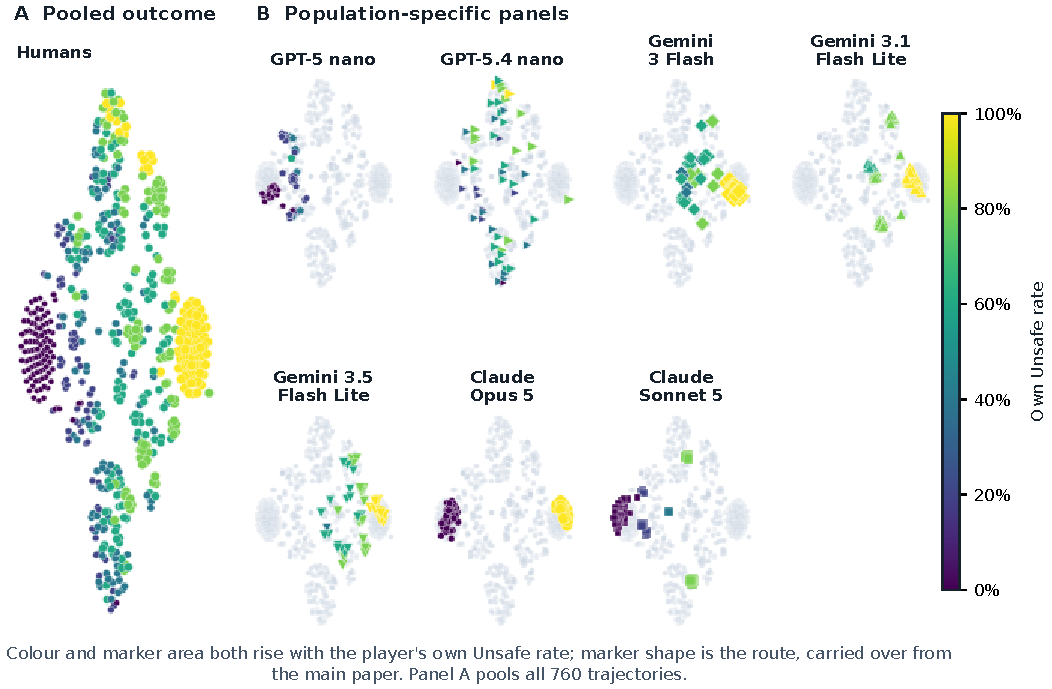
\includegraphics[width=\textwidth]{../figures/paper/llm_human_clustering/06_tsne_safe_unsafe.pdf}
    \caption{The same t-SNE coordinates as the population-identity embedding in the main paper,
    recoloured by each player's own mean \Unsafe{} rate over rounds 1--5
    (green = \Safe{}, red = \Unsafe{}) instead of population identity.
    Left: all 760 trajectories pooled. Right: the same colouring broken out
    per population.}
    \label{fig:human-tsne-outcome}
    \Description{The same t-SNE coordinates as the previous figure,
    recoloured by each player's own mean Unsafe rate over rounds 1 to 5
    rather than by which population produced it, on a green-to-red scale
    where green is Safe and red is Unsafe. The left panel pools all 760
    trajectories and the right panel breaks the same colouring out per
    population. The embedding separates almost entirely by Unsafe rate: a
    solid green region, a solid red region, and a mixed band between them,
    with very few red points inside the green region or the reverse.}
\end{figure*}



\subsection{Mean round-by-round profile per population}
\label{app:human-radar}

The embedding in the main paper shows that human trajectories spread more
widely than any single model's. This is the same comparison read one
feature at a time: population means over the fourteen features every
trajectory shares, with action probabilities and absolute progress gaps separated so
that neither scale obscures the other.

\begin{figure*}[t]
    \centering
    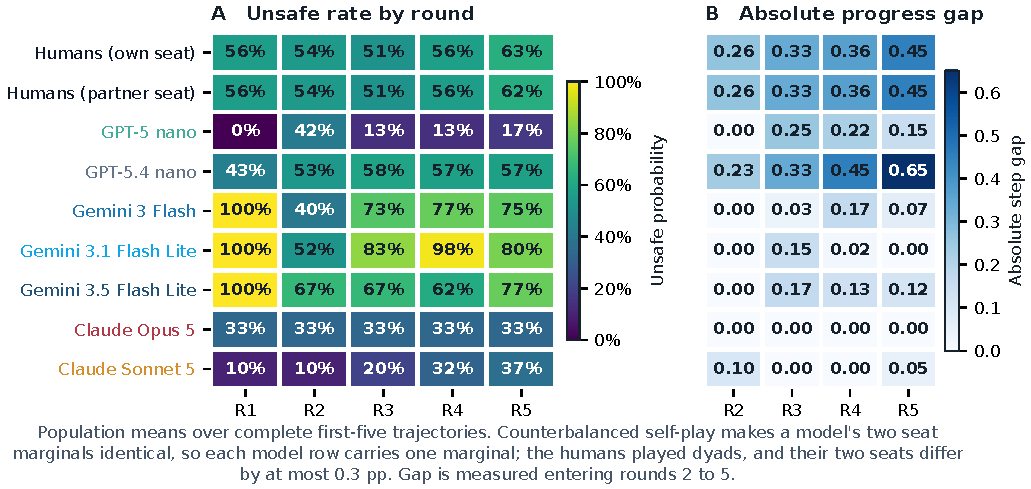
\includegraphics[width=\textwidth]{../figures/paper/llm_human_clustering/03_radar_small_multiples_by_group_no_gap_r1.pdf}
    \caption{Round-by-round profile for each population, shown as two
    source-backed heatmaps. Panel A reports the probability of an Unsafe
    action for each player's own and opponent action at rounds 1--5. Panel B
    reports the mean absolute progress gap entering rounds 2--5, so it
    measures how far apart the two players are after pooling focal-player
    roles. The eight rows are the human reference and the seven baseline
    model populations.}
    \label{fig:human-radar}
    \Description{Two heatmaps summarising fourteen shared trajectory
    features. The first heatmap gives Unsafe-action probabilities for own and
    opponent actions at five rounds. The second gives mean absolute progress
    gaps entering rounds two through five. Rows represent Human and seven
    model populations; red indicates more Unsafe action in the first panel,
    while darker blue indicates a larger separation in the second.}
\end{figure*}



\subsection{Unsafe rate by persona band and relative position}
\label{app:position-cells}

The main paper plots these rates as grouped bars for both checkpoints and
reports the pattern they show. The tables below give the cell-level numbers
behind that figure, so a single rate, its sample size and its confidence
interval can be checked directly.

\begin{table}[t]
    \caption{\Unsafe{} rate by persona band and relative position,
    GPT-5-nano. $n$ is the number of decisions in the cell; CI is the
    95\% confidence interval on the unsafe rate.}
    \label{tab:position-gpt5nano}
    \centering
    \small
    \begin{tabular}{@{}llrrl@{}}
        \toprule
        Persona band & Position & $n$ & \Unsafe{} rate & 95\% CI \\
        \midrule
        Baseline      & Leader  & 1460 & 19.7\% & 17.7--21.8\% \\
        Baseline      & Middle  & 1065 & 30.4\% & 27.7--33.3\% \\
        Baseline      & Trailer & 175  & 33.1\% & 26.6--40.4\% \\
        Low (R1--R2)  & Leader  & 1094 & 5.9\%  & 4.6--7.4\%   \\
        Low (R1--R2)  & Middle  & 198  & 14.6\% & 10.4--20.2\% \\
        Low (R1--R2)  & Trailer & 58   & 12.1\% & 6.0--22.9\%  \\
        Mid (R3--R4)  & Leader  & 649  & 40.7\% & 37.0--44.5\% \\
        Mid (R3--R4)  & Middle  & 451  & 38.1\% & 33.8--42.7\% \\
        Mid (R3--R4)  & Trailer & 250  & 32.8\% & 27.3--38.8\% \\
        High (R5--R6) & Leader  & 702  & 63.2\% & 59.6--66.7\% \\
        High (R5--R6) & Middle  & 339  & 54.3\% & 49.0--59.5\% \\
        High (R5--R6) & Trailer & 309  & 50.2\% & 44.6--55.7\% \\
        \bottomrule
    \end{tabular}
\end{table}


\begin{table}[t]
    \caption{\Unsafe{} rate by persona band and relative position,
    GPT-5.4-nano. Cells marked $^\dagger$ have $n<20$.}
    \label{tab:position-gpt54nano}
    \centering
    \small
    \begin{tabular}{@{}llrrl@{}}
        \toprule
        Persona band & Position & $n$ & \Unsafe{} rate & 95\% CI \\
        \midrule
        Baseline      & Leader  & 1649 & 83.6\%  & 81.8--85.3\%  \\
        Baseline      & Middle  & 703  & 84.8\%  & 81.9--87.2\%  \\
        Baseline      & Trailer & 348  & 86.5\%  & 82.5--89.7\%  \\
        Low (R1--R2)  & Leader  & 1073 & 3.3\%   & 2.4--4.5\%    \\
        Low (R1--R2)  & Middle  & 268  & 1.5\%   & 0.6--3.8\%    \\
        Low (R1--R2)  & Trailer & 9$^\dagger$    & 0.0\%   & 0.0--29.9\%   \\
        Mid (R3--R4)  & Leader  & 1164 & 95.7\%  & 94.4--96.7\%  \\
        Mid (R3--R4)  & Middle  & 70   & 88.6\%  & 79.0--94.1\%  \\
        Mid (R3--R4)  & Trailer & 116  & 91.4\%  & 84.9--95.3\%  \\
        High (R5--R6) & Leader  & 1328 & 99.3\%  & 98.7--99.6\%  \\
        High (R5--R6) & Middle  & 4$^\dagger$    & 100.0\% & 51.0--100.0\% \\
        High (R5--R6) & Trailer & 18$^\dagger$   & 100.0\% & 82.4--100.0\% \\
        \bottomrule
    \end{tabular}
\end{table}




\subsection{Behavioural-archetype coverage by population}
\label{app:archetype-coverage}

The main paper reports that human trajectories spread across more archetypes
than any single checkpoint's do. This table is the per-population breakdown
behind that statement, so a single share can be checked against its
population and archetype.

\begin{table}[t]
  \caption{Behavioural-archetype coverage: share of each population's
  neutral-lane player-races assigned to each human-fit archetype.
  Human row is the reference clustering ($n{=}341$); each LLM row
  projects that checkpoint's own no-persona player-races
  ($n{=}60$ to $120$) into the same
  space. The sample sizes are summarized in the evidence-strata table in the
  main paper. This table draws on the full nine-checkpoint cross-model pilot
  and therefore includes GPT-5.6 Luna and Terra, which are not part of
  the seven-model t-SNE/trajectory comparison earlier in
  this subsection.}
  \label{tab:archetype-coverage}
  \centering
  \footnotesize
  \setlength{\tabcolsep}{3pt}
  \begin{tabular}{@{}lrrrr@{}}
    \toprule
    Population & Cautious & Aggr./recip. & Catch-up & Persister \\
    \midrule
    Human (reference)      & 39.0\% & 49.9\% & 5.6\%  & 5.6\% \\
    GPT-5-nano              & 99.2\% & 0\%    & 0\%    & 0.8\% \\
    GPT-5.4-nano            & 51.7\% & 33.3\% & 3.3\%  & 11.7\% \\
    Gemini-3-Flash          & 1.7\%  & 78.3\% & 20.0\% & 0\% \\
    Gemini-3.1-Flash-Lite   & 0\%    & 83.3\% & 16.7\% & 0\% \\
    Gemini-3.5-Flash-Lite   & 0\%    & 76.7\% & 23.3\% & 0\% \\
    GPT-5.6 Luna            & 3.3\%  & 72.5\% & 24.2\% & 0\% \\
    GPT-5.6 Terra           & 14.2\% & 59.2\% & 26.7\% & 0\% \\
    Claude Opus 5           & 66.7\% & 33.3\% & 0\%    & 0\% \\
    Claude Sonnet 5         & 77.5\% & 20.8\% & 1.7\%  & 0\% \\
    \bottomrule
  \end{tabular}
\end{table}


\bibliographystyle{ACM-Reference-Format}
% \bibliography{sample}
\bibliography{references}


%%%%%%%%%%%%%%%%%%%%%%%%%%%%%%%%%%%%%%%%%%%%%%%%%%%%%%%%%%%%%%%%%%%%%%%%

\end{document}
